
\section{Transformaciones}

\begin{frame}
	\frametitle{Transformación a distribución normal}
		
		\begin{columns}
			
			% Columna de la izquierda
			\begin{column}{0.5\textwidth} % Ajusta la proporción según necesites
				\begin{figure}
					\centering
					\includegraphics[width=\textwidth]{hist_normal_rice} % Asegúrate de cambiar la ruta a la ubicación de tu imagen
					\caption{Histograma de distribución normal.}
				\end{figure}
			\end{column}
			
			% Columna de la derecha
			\begin{column}{0.5\textwidth} % Ajusta la proporción según necesites
				\begin{itemize}
					\item La transformación de una distribución uniforme a normal se realiza mediante la función de error inversa.
					\item Convierte cuantiles uniformes en valores de una distribución normal, ajustándolos después según la media y desviación estándar deseadas.
					\item Facilita la interpretación estadística, mapeando probabilidades uniformes a la escala de la normalidad.
				\end{itemize}
			\end{column}
		\end{columns}
\end{frame}


\begin{frame}
	\frametitle{Transformación a distribución gamma}
	
	\begin{columns}
		% Columna de la derecha
		\begin{column}{0.5\textwidth} % Ajusta la proporción según necesites
			\begin{itemize}
				\item El método de aceptación-rechazo genera variables aleatorias Gamma a partir de distribuciones uniformes. 
				\item Se calcula un valor \(y\) a partir de una variable uniforme y se compara con una función de densidad proporcional a la distribución Gamma. Si \(y\) es aceptado según un criterio de comparación, se escala y se retorna como resultado.
			\end{itemize}
			
		\end{column}

	
	
	% Columna de la izquierda
	\begin{column}{0.5\textwidth} % Ajusta la proporción según necesites
		\begin{figure}
			\centering
			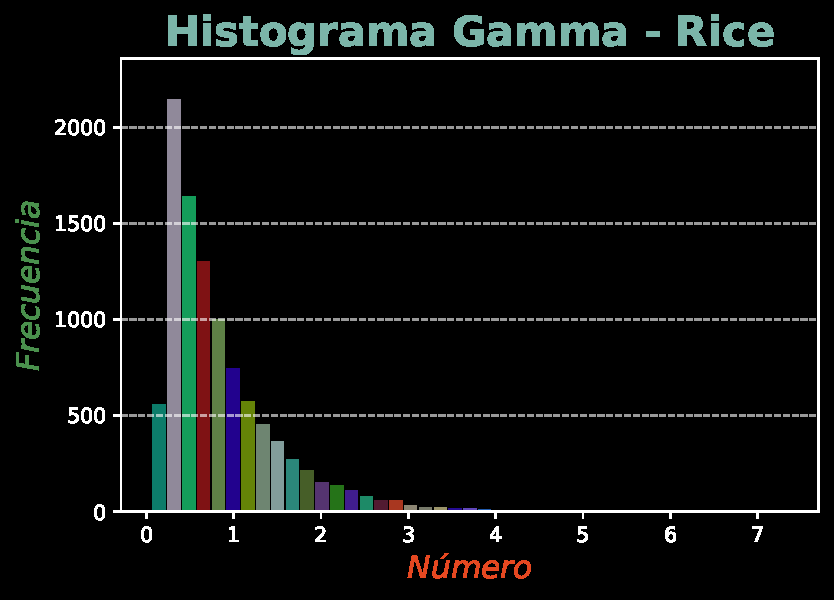
\includegraphics[width=\textwidth]{hist_gamma_Rice} % Asegúrate de cambiar la ruta a la ubicación de tu imagen
			\caption{Histograma de distribución gamma.}
		\end{figure}
	\end{column}
	\end{columns}
\end{frame}


\begin{frame}
	\frametitle{Transformación lineal}
	
	\begin{columns}
		
		% Columna de la izquierda
		\begin{column}{0.5\textwidth} % Ajusta la proporción según necesites
			\begin{figure}
				\centering
				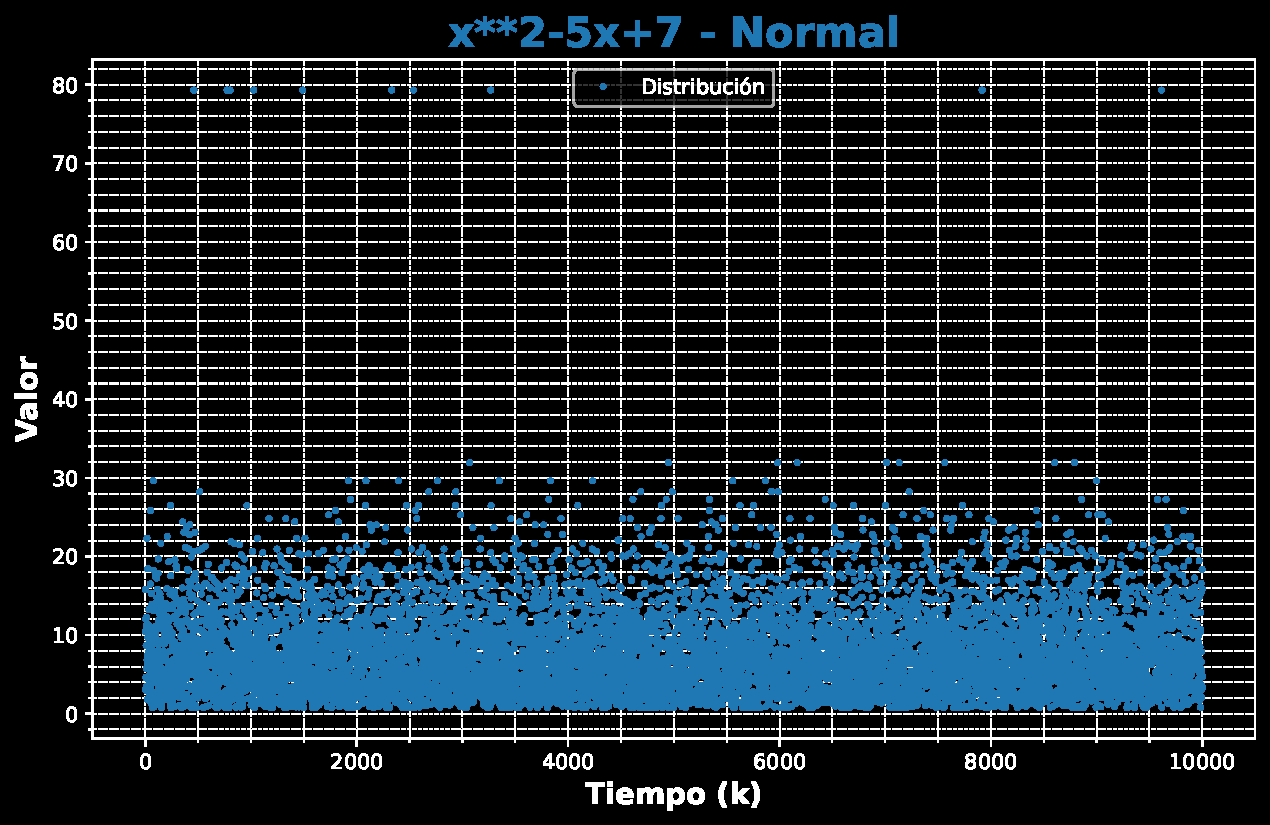
\includegraphics[width=\textwidth]{cuad_normal1} % Asegúrate de cambiar la ruta a la ubicación de tu imagen
				\caption{Gráfica de la serie de tiempo para el polinomio $x^2-5x+7$.}
			\end{figure}
		\end{column}
		
		% Columna de la derecha
		\begin{column}{0.5\textwidth} % Ajusta la proporción según necesites
			\begin{figure}
				\centering
				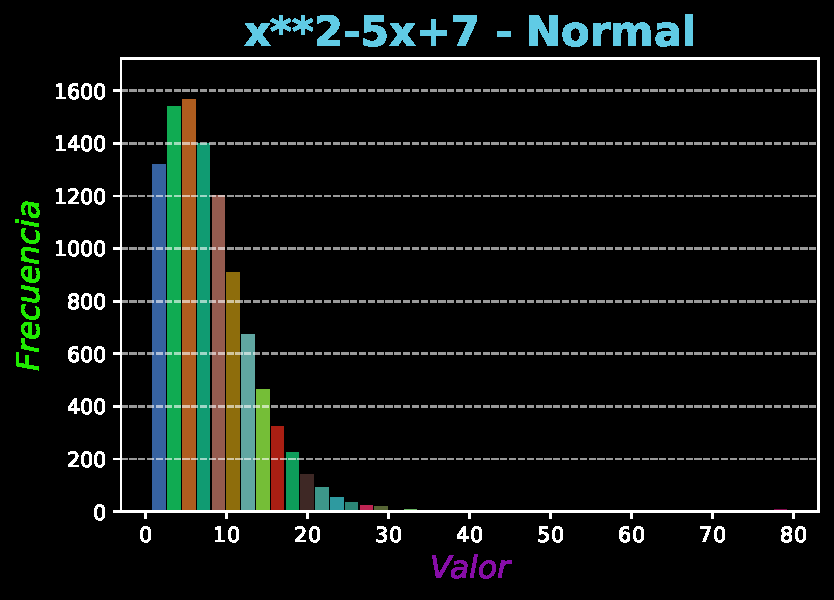
\includegraphics[width=\textwidth]{cuad_normal2} % Asegúrate de cambiar la ruta a la ubicación de tu imagen
				\caption{Distribución de los datos.}
			\end{figure}
		\end{column}
	\end{columns}
\end{frame}


\begin{frame}
	\frametitle{Transformación no lineal}
	
	\begin{columns}
		
		% Columna de la izquierda
		\begin{column}{0.5\textwidth} % Ajusta la proporción según necesites
			\begin{figure}
				\centering
				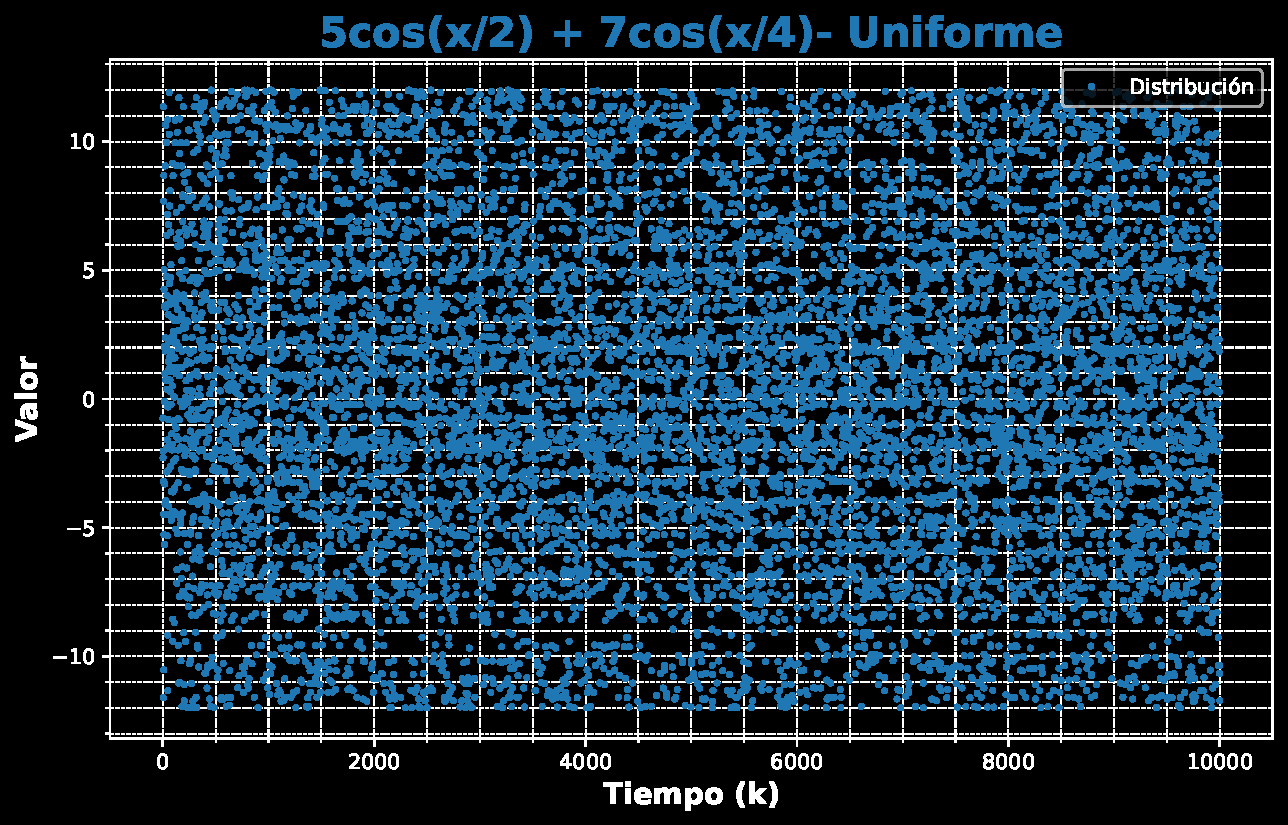
\includegraphics[width=\textwidth]{per_uniforme1} % Asegúrate de cambiar la ruta a la ubicación de tu imagen
				\caption{Gráfica de la serie de tiempo para la función \( 5\cdot \cos\left(\frac{x}{2}\right) + 7\cdot \cos\left(\frac{x^2}{4}\right) \).}
			\end{figure}
		\end{column}
		
		% Columna de la derecha
		\begin{column}{0.5\textwidth} % Ajusta la proporción según necesites
			\begin{figure}
				\centering
				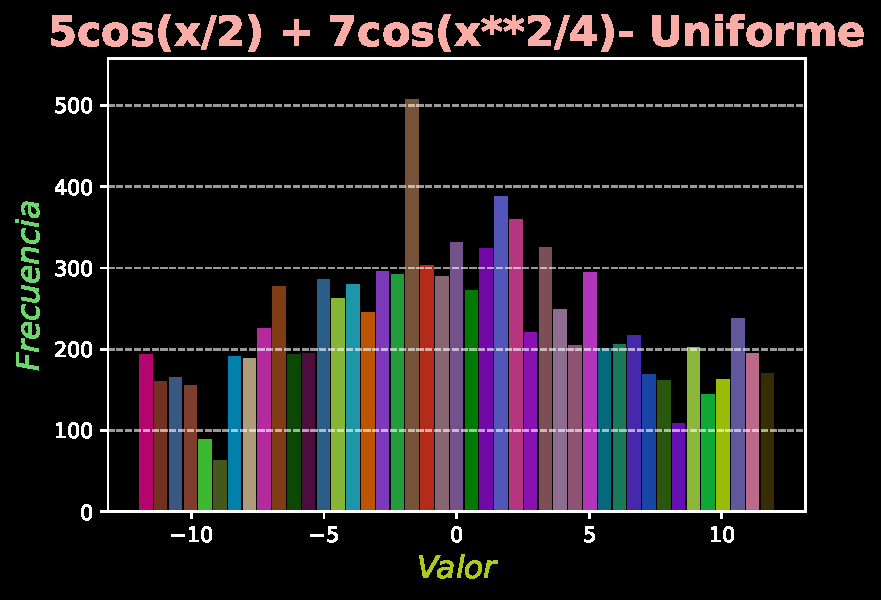
\includegraphics[width=\textwidth]{per_uniforme2} % Asegúrate de cambiar la ruta a la ubicación de tu imagen
				\caption{Distribución de los datos.}
			\end{figure}
		\end{column}
	\end{columns}
\end{frame}


%------------------------------------------------

